\section{强大数律}
\label{sec:lln-strong-law}

弱大数律对每个固定的$n$说：偏差超过$\varepsilon$的路径只占很小的比例。它没有说同一条路径以后不会再出界。图~\ref{fig:lln-weak-vs-strong}画出$40$条硬币频率路径（种子$21$）与带$0.5\pm0.05$。在$n=400$处只有$3$条在带外，这是弱大数律描述的事情。另一个问题是：沿着一条固定的路径往后看，它是否从某一步起永远留在带内？图中红点标出每条路径在$n\leq2000$内最后一次出带的时刻，最晚的在$n=727$。

\begin{BookInlineFigure}
 \centering
 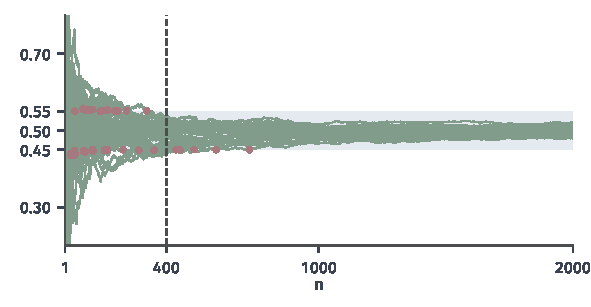
\includegraphics[width=100mm]{figures/07-probability/03-probability-limits/matplotlib/lln-weak-vs-strong/figure.pdf}
 \caption{$40$条均匀硬币的频率路径（绿线，种子$21$），$n\leq2000$。浅蓝带为$0.5\pm0.05$；红点为各路径在图示范围内最后一次位于带外的时刻；虚线标出$n=400$。}
 \label{fig:lln-weak-vs-strong}
\end{BookInlineFigure}

图只能显示有限的范围，“永远留在带内”是关于整条无限路径的断言。把它写成定义，就是几乎必然收敛。

\begin{definition}[强大数律]
\label{def:lln-strong-law}
设随机变量列$X_1,X_2,\dots$各项可积且有共同的均值$\mu$。若$\bar{X}_n\xrightarrow{\mathrm{a.s.}}\mu$，即
\begin{equation}
 \mathbb{P}\Bigl(\lim_{n\to\infty}\bar{X}_n=\mu\Bigr)=1 ,
 \label{eq:lln-strong-law}
\end{equation}
则称这列变量满足\term{强大数律}（strong law of large numbers）。
\end{definition}

由第~\ref{chap:random-variable-convergence}章，几乎必然收敛蕴含依概率收敛，所以强律推出弱律。反过来不能直接升级。Chebyshev界$\sigma^2/(n\varepsilon^2)$对$n$求和发散，Borel–Cantelli引理无从使用：每个时刻出界的概率虽小，加起来却是无穷，不能排除无穷多次出界。要证明强律，需要同时控制所有后续时刻，这正是前两节为随机级数建立的工具。思路是先证明加权级数$\sum_k(X_k-\mu)/k$收敛，再把级数的收敛翻译成平均的收敛。

\subsection{从级数收敛到平均收敛}
\label{sec:lln-series-to-average}

先看一个确定的问题。设实数$x_1,x_2,\dots$使$\sum_kx_k/k$收敛，能否推出$\frac1n\sum_{k\leq n}x_k\to0$？直觉是：级数收敛说明$x_k$按自身大小$k$折算后的累计有限，而前$n$项的总和除以更大的$n$时，早期各项被压小，后期各项又已经很小。

\begin{lemma}[Kronecker引理]
\label{lem:lln-kronecker}
设$0<b_1\leq b_2\leq\cdots$，$b_n\to\infty$，实数列$(x_k)$使$\sum_kx_k/b_k$收敛。则
\begin{equation}
 \lim_{n\to\infty}\frac{1}{b_n}\sum_{k=1}^{n}x_k=0 .
 \label{eq:lln-kronecker}
\end{equation}
\end{lemma}

这个结论称为\term{Kronecker引理}（Kronecker's lemma）。证明用\term{分部求和}（summation by parts），即离散形式的分部积分。

\begin{proof}
记$s_0=0$，$s_n=\sum_{k\leq n}x_k/b_k$，由假设$s_n\to s$。于是$x_k=b_k(s_k-s_{k-1})$。分部求和，把$b_k$与差分$s_k-s_{k-1}$交换位置：
\[
 \sum_{k=1}^{n}x_k=\sum_{k=1}^{n}b_k(s_k-s_{k-1})=b_ns_n-\sum_{k=1}^{n-1}(b_{k+1}-b_k)s_k .
\]
这个恒等式可以按$s_k$的系数逐项核对：$s_n$的系数是$b_n$，$k<n$时$s_k$的系数是$b_k-b_{k+1}$。两边除以$b_n$，
\begin{equation}
 \frac{1}{b_n}\sum_{k=1}^{n}x_k=s_n-\frac{1}{b_n}\sum_{k=1}^{n-1}(b_{k+1}-b_k)s_k .
 \label{eq:lln-abel-identity}
\end{equation}

右边第二项是$s_1,\dots,s_{n-1}$的加权平均，权重$w_{n,k}=(b_{k+1}-b_k)/b_n\geq0$，总和为$(b_n-b_1)/b_n\to1$。下面说明它趋于$s$。给定$\eta>0$，取$N$使$k\geq N$时$\lvert s_k-s\rvert<\eta$。则$n>N$时
\[
 \Bigl\lvert\sum_{k=1}^{n-1}w_{n,k}(s_k-s)\Bigr\rvert\leq\frac{1}{b_n}\sum_{k=1}^{N-1}(b_{k+1}-b_k)\lvert s_k-s\rvert+\eta .
\]
右边第一项的分子与$n$无关，$b_n\to\infty$时趋于零。所以上极限不超过$\eta$，而$\eta$任意。再由$\sum_kw_{n,k}s=s(b_n-b_1)/b_n\to s$，第二项趋于$s$。式~\eqref{eq:lln-abel-identity}的右边趋于$s-s=0$。
\end{proof}

$b_n=n$时，$b_{k+1}-b_k=1$，式~\eqref{eq:lln-abel-identity}的加权平均就是$\frac1n\sum_{k<n}s_k$，即部分和序列的\term{Cesàro平均}（Cesàro mean）。证明的核心是：收敛序列的Cesàro平均收敛到同一极限，而样本平均恰好是原序列与它的Cesàro平均之差。

\paragraph{一个确定的例子}
取$x_k=(-1)^{k+1}\sqrt{k}$。$\sum_kx_k/k=\sum_k(-1)^{k+1}/\sqrt{k}$是交错级数，项的绝对值单调趋于零，所以收敛，和约为$0.6049$。由Kronecker引理，
\[
 \frac1n\sum_{k=1}^{n}(-1)^{k+1}\sqrt{k}\to0 .
\]
直接计算，$n=100,1000,10000$时这个平均分别约为$-0.0463$、$-0.0154$、$-0.0050$，大致与$-1/(2\sqrt{n})$相当。注意$x_k$本身无界，$\lvert x_k\rvert=\sqrt{k}\to\infty$，平均趋于零完全来自正负抵消。

图~\ref{fig:lln-kronecker}画出式~\eqref{eq:lln-abel-identity}中的两项。图(a)中蓝线$s_n$来回振荡地收敛，黄线是它的Cesàro平均，平滑地趋于同一极限；图(b)是二者之差，即样本平均，它被夹在$\pm1/(2\sqrt{n})$之间趋于零。

\begin{BookInlineFigure}
 \centering
 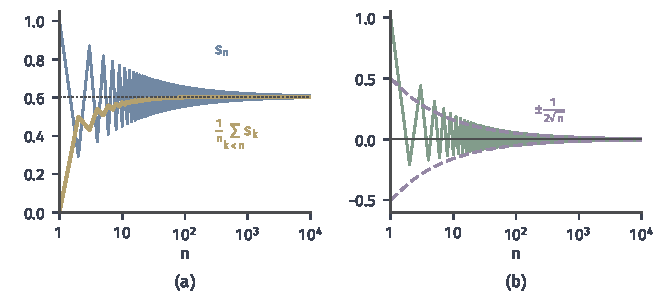
\includegraphics[width=112mm]{figures/07-probability/03-probability-limits/matplotlib/lln-kronecker/figure.pdf}
 \caption{Kronecker引理的恒等式~\eqref{eq:lln-abel-identity}，$b_n=n$，$x_k=(-1)^{k+1}\sqrt{k}$，横轴为对数刻度。(a)$s_n=\sum_{k\leq n}x_k/k$（蓝线）与其Cesàro平均$\frac1n\sum_{k<n}s_k$（黄线），点线为极限$0.6049$；(b)二者之差$\frac1n\sum_{k\leq n}x_k$（绿线）与$\pm1/(2\sqrt{n})$（紫色虚线）。}
 \label{fig:lln-kronecker}
\end{BookInlineFigure}

\paragraph{用到随机变量上}
Kronecker引理是关于实数列的确定性结论。用于随机变量时，先找一个概率为一的事件，在它上面级数收敛，再对其中每个样本点分别使用引理。下面的定理就是这样得到的。

\begin{theorem}[方差加权可和时的强大数律]
\label{thm:lln-kolmogorov-criterion}
设$X_1,X_2,\dots$相互独立，$\mu_k=\mathbb{E}[X_k]$，$\sigma_k^2=\operatorname{Var}(X_k)$，且
\begin{equation}
 \sum_{k=1}^{\infty}\frac{\sigma_k^2}{k^2}<\infty .
 \label{eq:lln-kolmogorov-criterion}
\end{equation}
则
\begin{equation}
 \frac{\tilde{S}_n}{n}=\frac1n\sum_{k=1}^{n}(X_k-\mu_k)\xrightarrow{\mathrm{a.s.}}0 .
 \label{eq:lln-kolmogorov-slln}
\end{equation}
\end{theorem}

\begin{proof}
变量$(X_k-\mu_k)/k$相互独立，均值为零，方差为$\sigma_k^2/k^2$。由条件~\eqref{eq:lln-kolmogorov-criterion}与定理~\ref{thm:lln-variance-series}，存在概率为一的事件$\Omega_0$，在其上级数$\sum_k(X_k-\mu_k)/k$收敛。对每个$\omega\in\Omega_0$，对实数列$x_k=X_k(\omega)-\mu_k$与$b_k=k$用引理~\ref{lem:lln-kronecker}，得到$\tilde{S}_n(\omega)/n\to0$。
\end{proof}

两个特例直接可用。第一，独立同分布且方差$\sigma^2$有限时，$\sum_k\sigma^2/k^2<\infty$，所以$\bar{X}_n\xrightarrow{\mathrm{a.s.}}\mu$：有限方差的强大数律成立。第二，第~\ref{sec:lln-normalization}小节的分段Bernoulli变量满足$\sigma_k^2=p_k(1-p_k)\leq1/4$，条件成立，所以$(S_n-\sum_{k\leq n}p_k)/n\to0$几乎必然成立，这正是图~\ref{fig:lln-varying-means}(b)显示的现象。各项分布不同，样本平均本身却不收敛，强律的正确形式是中心化平均趋于零。

\subsection{独立同分布可积情形}
\label{sec:lln-slln-integrable}

最后去掉有限方差的假设。与弱律一样，办法是截断；不同的是，截断水平这次随项数增长。

\begin{theorem}[强大数律]
\label{thm:lln-slln}
设$X_1,X_2,\dots$独立同分布，$\mathbb{E}[\lvert X_1\rvert]<\infty$，$\mu=\mathbb{E}[X_1]$。则$\bar{X}_n\xrightarrow{\mathrm{a.s.}}\mu$。
\end{theorem}

\begin{proof}
对每个$k$，在水平$k$处截断：
\[
 Y_k=X_k\mathbf{1}_{\{\lvert X_k\rvert\leq k\}} .
\]
$Y_k$是独立变量$X_k$的函数，所以$Y_1,Y_2,\dots$相互独立，但截断水平不同，它们不再同分布。把样本平均的偏差拆成三项：
\[
 \bar{X}_n-\mu=\frac1n\sum_{k=1}^{n}(X_k-Y_k)+\frac1n\sum_{k=1}^{n}\bigl(Y_k-\mathbb{E}[Y_k]\bigr)+\Bigl(\frac1n\sum_{k=1}^{n}\mathbb{E}[Y_k]-\mu\Bigr) .
\]
下面分三步证明每一项几乎必然趋于零。

\emph{第一步：大项只出现有限次。}$X_k$与$X_1$同分布，所以$X_k\neq Y_k$的概率是$\mathbb{P}(\lvert X_1\rvert>k)$。函数$t\mapsto\mathbb{P}(\lvert X_1\rvert>t)$不增，所以它在$t=k$处的值不超过它在区间$[k-1,k]$上的平均：
\[
 \mathbb{P}(\lvert X_1\rvert>k)\leq\int_{k-1}^{k}\mathbb{P}(\lvert X_1\rvert>t)\,\mathrm{d}t .
\]
对$k$求和，再由第~\ref{chap:tail-probabilities}章的尾积分公式，
\[
 \sum_{k=1}^{\infty}\mathbb{P}(\lvert X_1\rvert>k)\leq\int_0^{\infty}\mathbb{P}(\lvert X_1\rvert>t)\,\mathrm{d}t=\mathbb{E}[\lvert X_1\rvert]<\infty .
\]
由Borel–Cantelli引理，几乎必然只有有限个$k$使$X_k\neq Y_k$。在这样的样本点上，$\sum_{k\leq n}(X_k-Y_k)$从某项起不再变化，除以$n$后趋于零。

\emph{第二步：截断均值趋于$\mu$。}由同分布，$\mathbb{E}[Y_k]$等于$X_1\mathbf{1}_{\{\lvert X_1\rvert\leq k\}}$的期望。这个随机变量逐点趋于$X_1$，且被可积的$\lvert X_1\rvert$控制，由支配收敛定理$\mathbb{E}[Y_k]\to\mu$。收敛数列的Cesàro平均收敛到同一极限（这是Kronecker引理证明中的第二步，取$b_n=n$），所以第三项趋于零。

\emph{第三步：截断波动的加权方差可和。}要对$Y_k-\mathbb{E}[Y_k]$用定理~\ref{thm:lln-kolmogorov-criterion}，需检查$\sum_k\operatorname{Var}(Y_k)/k^2<\infty$。由$\operatorname{Var}(Y_k)\leq\mathbb{E}[Y_k^2]$，并交换非负项的求和与期望，
\[
 \sum_{k=1}^{\infty}\frac{\operatorname{Var}(Y_k)}{k^2}\leq\sum_{k=1}^{\infty}\frac{\mathbb{E}\bigl[X_1^2\mathbf{1}_{\{\lvert X_1\rvert\leq k\}}\bigr]}{k^2}=\mathbb{E}\Bigl[X_1^2\sum_{k\geq\lvert X_1\rvert,\,k\geq1}\frac{1}{k^2}\Bigr] .
\]
对实数$x\neq0$，记$m=\lceil\lvert x\rvert\rceil\geq1$，则$m\geq\lvert x\rvert$，并且
\[
 \sum_{k\geq m}\frac{1}{k^2}\leq\frac{1}{m^2}+\int_m^{\infty}\frac{\mathrm{d}t}{t^2}=\frac{1}{m^2}+\frac1m\leq\frac2m\leq\frac{2}{\lvert x\rvert} .
\]
所以期望内的量不超过$x^2\cdot2/\lvert x\rvert=2\lvert x\rvert$；$x=0$时它为零。于是
\[
 \sum_{k=1}^{\infty}\frac{\operatorname{Var}(Y_k)}{k^2}\leq2\,\mathbb{E}[\lvert X_1\rvert]<\infty .
\]
由定理~\ref{thm:lln-kolmogorov-criterion}，第二项几乎必然趋于零。

三项各在一个概率为一的事件上趋于零，三个事件的交概率仍为一，定理得证。
\end{proof}

\paragraph{为什么截断水平取$k$}
若在固定水平$c$截断，被截掉的大值以固定概率$\mathbb{P}(\lvert X_1\rvert>c)>0$反复出现，无穷多次，第一步失效。若截断水平增长得太快，截断变量的方差太大，第三步的级数可能发散。水平$k$恰好使两边都只用到一阶矩：第一步的级数$\sum_k\mathbb{P}(\lvert X_1\rvert>k)$与第三步的级数都被$\mathbb{E}[\lvert X_1\rvert]$控制。

用$\alpha=1.5$的Pareto分布核对两个级数。第一步，$\mathbb{P}(X_1>k)=k^{-1.5}$，
\[
 \sum_{k=1}^{\infty}k^{-1.5}\approx2.612\leq\mathbb{E}[X_1]=3 .
\]
第三步，$\mathbb{E}[Y_k^2]=3(\sqrt{k}-1)$，
\[
 \sum_{k=1}^{\infty}\frac{3(\sqrt{k}-1)}{k^2}\approx2.896\leq2\,\mathbb{E}[X_1]=6 .
\]
图~\ref{fig:lln-truncation-diagonal}画出一组$2000$个Pareto观测（种子$17$）与对角线$x=k$。落在对角线上方、被截断改动的只有$5$个点，位于$k=1,2,10,19,335$；按第一步的级数，期望个数约为$2.57$。$k$越大，越过$k$越难，这些点集中在开头。

\begin{BookInlineFigure}
 \centering
 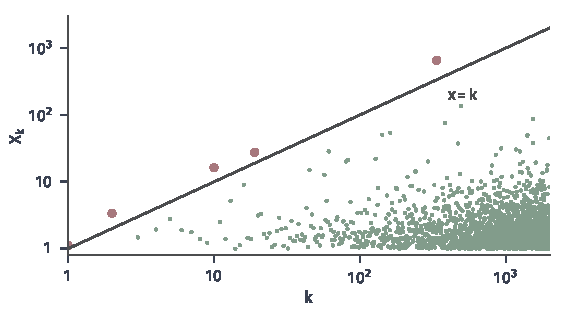
\includegraphics[width=96mm]{figures/07-probability/03-probability-limits/matplotlib/lln-truncation-diagonal/figure.pdf}
 \caption{$\alpha=1.5$的Pareto样本$X_1,\dots,X_{2000}$（种子$17$），双对数坐标。深灰直线为截断水平$x=k$；红点为$X_k>k$、被截断改动的观测，绿点为其余观测。}
 \label{fig:lln-truncation-diagonal}
\end{BookInlineFigure}

\paragraph{可积条件不能去掉}
对独立同分布序列，可积性不仅充分，而且必要。设$\mathbb{E}[\lvert X_1\rvert]=\infty$。与第一步反方向比较，$\mathbb{P}(\lvert X_1\rvert>k)$不小于生存函数在$[k,k+1]$上的平均，所以
\[
 \sum_{k=1}^{\infty}\mathbb{P}(\lvert X_k\rvert>k)\geq\int_1^{\infty}\mathbb{P}(\lvert X_1\rvert>t)\,\mathrm{d}t\geq\mathbb{E}[\lvert X_1\rvert]-1=\infty .
\]
事件$\{\lvert X_k\rvert>k\}$相互独立，由Borel–Cantelli引理的第二部分，几乎必然有无穷多个$k$使$\lvert X_k\rvert/k>1$。另一方面，若$\bar{X}_n$收敛到有限数$L$，则
\[
 \frac{X_n}{n}=\bar{X}_n-\frac{n-1}{n}\bar{X}_{n-1}\to L-L=0 .
\]
两者矛盾，所以$\bar{X}_n$收敛到有限极限的概率为零。图~\ref{fig:lln-pareto-cauchy}(b)的Cauchy路径就是这种情形。

\paragraph{弱律与强律的比较}
表~\ref{tab:lln-weak-strong}把两种大数律放在一起。对独立同分布序列，强律的条件恰好是可积；弱律的结论较弱，它在比可积稍弱的尾部条件下仍可能对适当的中心成立，读者可查阅~\scite{math-kallenberg2021probability}。

\begin{BookInlineTable}
 \centering
 \caption{弱大数律与强大数律（独立同分布，$\mu=\mathbb{E}[X_1]$）。}
 \label{tab:lln-weak-strong}
 \begin{tabular}{lll}
  \toprule
  & 弱大数律 & 强大数律\\
  \midrule
  结论 & 依概率收敛 & 几乎必然收敛\\
  控制对象 & 每个固定时刻 & 整条路径的尾部\\
  有限方差时 & Chebyshev不等式 & 加权级数与Kronecker引理\\
  只有一阶矩时 & 固定水平截断 & 水平随$k$增长的截断\\
  有限样本误差 & 有方差时为$\sigma^2/(n\varepsilon^2)$ & 本身不给速度\\
  \bottomrule
 \end{tabular}
\end{BookInlineTable}

强律回答的是“最终会不会稳定”，它本身不说明何时稳定，也不给出有限样本的误差。对固定的$n$，误差大小仍要靠Chebyshev不等式或更强的集中不等式估计；后者对有界变量给出指数衰减的界，可参考\BookChapterRef{chap:finite-sample-error-bounds}{卷八第4章“有限样本的误差上界”}。
